\section{Evaluation}
In this section the following algorithms will be used for classification:
\begin{itemize}
 \item Support Vector Machine
 \item Multi Layer Perceptron
 \item k-Nearest-Neighbor
 \item Normal Bayes
 \item Decision Tree
\end{itemize}

To evaluate a predictor it is possible to calculate its accuracy. For two classes it is given as:

$$Accuracy = \frac{\mbox{true positive}}{\mbox{true positive} + \mbox{false positive}}$$

The performance of Support Vector Machines and especially Neural Networks depend on the parameters chosen. In case of a neural network it is difficult to find the appropriate parameters and architecture. Designing an Artifical Neural Network is often more a rule of thumb and networks should be optimized iteratively starting with one hidden layer and few neurons. Parameters for a Support Vector Machine can be estimated using Cross Validation and Grid Search (both can be used as \lstinline|train_auto| in OpenCV $\geq$ 2.0).
 
Parameters are not optimized in this experiment, remember to optimize the parameters yourself when using one of the algorithms.

\subsection{Experiment Data}
In this experiment linear and non-linear functions are learned. $200$ points for training and $2000$ points for testing are generated.

\subsection{y = 2x}

\begin{center}
\begin{tabular}{|c|c|}
\hline
Predictor &	 Accuracy\\ \hline\hline
Support Vector Machine &	0.99\\ \hline
Multi Layer Perceptron (2, 10, 15, 1) & 0.994\\ \hline
k-Nearest-Neighbor (k = 3) & 0.9825\\ \hline
Normal Bayes &	0.9425 \\ \hline
Decision Tree &	0.923\\ \hline
\end{tabular}
\end{center}

\subsubsection{Plot}
\begin{center}
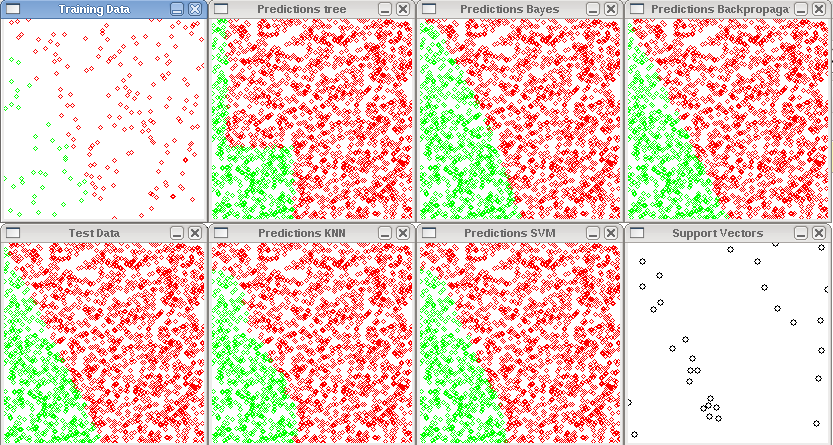
\includegraphics[scale=0.4]{img/eval/2x.png}
\end{center}

\subsection{y = sin(10x)}

\begin{center}
\begin{tabular}{|c|c|}
\hline
Predictor &	Accuracy\\ \hline\hline
Support Vector Machine &	0.913\\ \hline
Multi Layer Perceptron (2, 10, 15, 1) & 0.6855\\ \hline
k-Nearest-Neighbor (k = 3) & 0.9\\ \hline
Normal Bayes & 0.632\\ \hline
Decision Tree &	0.886\\ \hline
\end{tabular}
\end{center}

\subsubsection{Plot}
\begin{center}
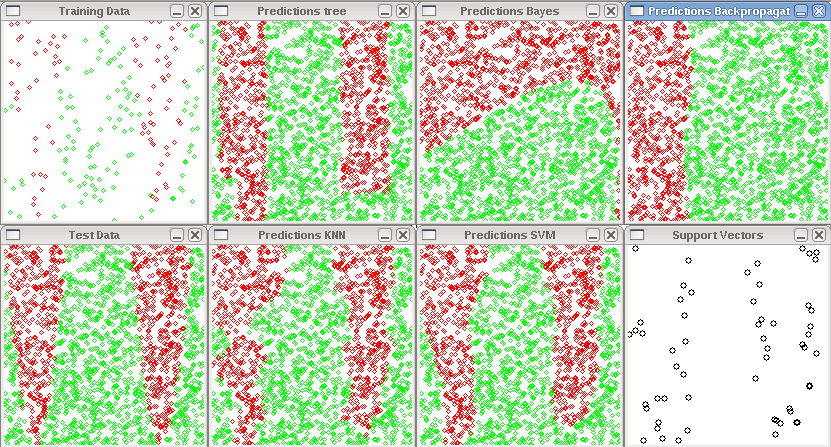
\includegraphics[scale=0.4]{img/eval/sin10x.png}
\end{center}

\subsection{y = tan(10x)}

\begin{center}
\begin{tabular}{|c|c|}
\hline
Predictor &	Accuracy\\ \hline\hline
Support Vector Machine & 0.7815\\ \hline
Multi Layer Perceptron (2, 10, 15, 1) &	0.5115\\ \hline
k-Nearest-Neighbor (k = 3) & 0.8195\\ \hline
Normal Bayes &	0.542\\ \hline
Decision Tree &	0.9155\\ \hline
\end{tabular}
\end{center}

\subsubsection{Plot}
\begin{center}
 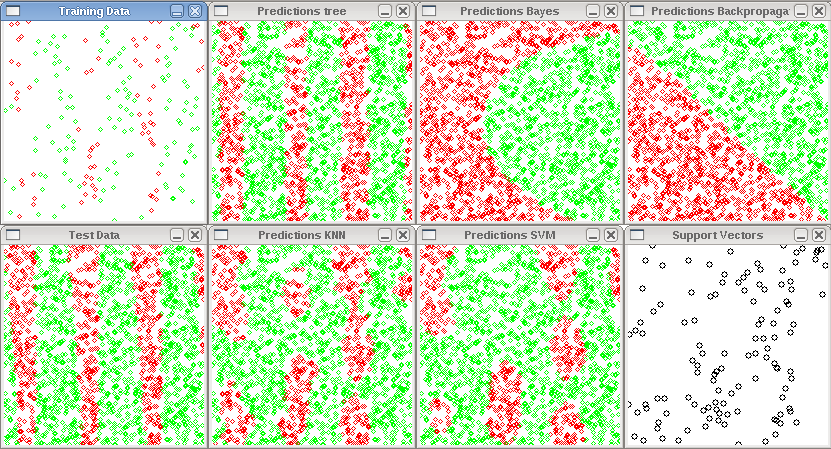
\includegraphics[scale=0.4]{img/eval/tan10x.png}
\end{center}
